% !TeX root = ../main.tex

\section{Numerical Results}
    \frame{\sectionpage}

    \begin{frame}{Running time of Benders Decomposition and IP}
        \tiny
        \begin{table}[ht]
            \centering
            \begin{tabular}{|l|l|l|l|l|l|l|}
            \hline
            \# of scenarios & demands & running time of IP(s) & Benders (s) & \# of rows & \# of groups & \# of seats\\
            \hline
            1000  & (150, 350) & 5.1  & 0.13 & 30 & 8 & (21, 50)\\
            5000  & & 28.73 & 0.47 & 30 & 8 & \\
            10000 & & 66.81  & 0.91 & 30 & 8 & \\
            50000 & & 925.17 & 4.3 & 30 & 8 & \\
            \hline
            1000  & (1000, 2000) & 5.88 & 0.29 & 200 & 8 & (21, 50)\\
            5000  & & 30.0 & 0.62 & 200 & 8 & \\
            10000 & & 64.41 & 1.09 & 200 & 8 & \\
            50000 & & 365.57 & 4.56 & 200 & 8 & \\
            \hline
            1000  & (150, 250) & 17.15  & 0.18 & 30 & 16 & (41, 60) \\
            5000  & & 105.2  & 0.67 & 30 & 16 & \\
            10000 & & 260.88 & 1.28 & 30 & 16 & \\
            50000 & & 3873.16 & 6.18 & 30 & 16 & \\
            \hline
            \end{tabular}
          \end{table}
    \end{frame}
      
    \begin{frame}{Feasible Seat Planning versus IP Solution}
        \scriptsize
        \begin{table}[ht]
            \begin{tabular}{|l|l|l|l|l|l|}
            \hline
            \# samples & T & probabilities & \# rows & people served by FSP & IP \\
            \hline
            1000  & 45  & [0.4,0.4,0.1,0.1] & 8 & 85.30 & 85.3 \\
            1000  & 50  & [0.4,0.4,0.1,0.1] & 8 & 97.32 & 97.32 \\
            1000  & 55  & [0.4,0.4,0.1,0.1] & 8 & 102.40 & 102.40  \\ % slow
            1000  & 60  & [0.4,0.4,0.1,0.1] & 8 & 106.70 & NA  \\
            1000  & 65  & [0.4,0.4,0.1,0.1] & 8 & 108.84 & 108.84 \\
            \hline
            1000  & 35  & [0.25,0.25,0.25,0.25] & 8 & 87.16 & 87.08 \\
            1000  & 40  & [0.25,0.25,0.25,0.25] & 8 & 101.32 & 101.24 \\
            1000  & 45  & [0.25,0.25,0.25,0.25] & 8 & 110.62 & 110.52 \\
            1000  & 50  & [0.25,0.25,0.25,0.25] & 8 & 115.46 & NA \\
            1000  & 55  & [0.25,0.25,0.25,0.25] & 8 & 117.06 & 117.26 \\
            \hline
            5000  & 300  & [0.25,0.25,0.25,0.25] & 30 & 749.76 & 749.76 \\
            5000  & 350  & [0.25,0.25,0.25,0.25] & 30 & 866.02 & 866.42 \\
            5000  & 400  & [0.25,0.25,0.25,0.25] & 30 & 889.02 & 889.44 \\
            5000  & 450  & [0.25,0.25,0.25,0.25] & 30 & 916.16 & 916.66 \\
            \hline
            \end{tabular}
        \end{table}

    Each entry of people served is the average of 50 instances.
    IP will spend more than 2 hours in some instances, as `NA' showed in the table.
    \end{frame}
      
    \begin{frame}{Performances of Different Policies}
        \scriptsize
        \begin{table}[ht]
          \centering
          \begin{tabular}{|l|l|l|l|l|l|l|}
          \hline
           T & Probabilities & SPP(\%) & DP1(\%) & Bid(\%) & Booking(\%) & FCFS(\%) \\
          \hline
          60  & [0.25, 0.25, 0.25, 0.25]  & 99.12 & 98.42 & 98.38 & 96.74 & 98.17 \\
          70  & [0.25, 0.25, 0.25, 0.25]  & 98.34 & 96.87 & 96.24 & 97.18 & 94.75 \\
          80  & [0.25, 0.25, 0.25, 0.25]  & 98.61 & 95.69 & 96.02 & 98.00 & 93.18 \\
          90  & [0.25, 0.25, 0.25, 0.25]  & 99.10 & 96.05 & 96.41 & 98.31 & 92.48 \\
          100 & [0.25, 0.25, 0.25, 0.25]  & 99.58 & 95.09 & 96.88 & 98.70 & 92.54 \\
          \hline
          60  & [0.25, 0.35, 0.05, 0.35]  & 98.94 & 98.26 & 98.25 & 96.74 & 98.62 \\
          70  & [0.25, 0.35, 0.05, 0.35]  & 98.05 & 96.62 & 96.06 & 96.90 & 93.96 \\
          80  & [0.25, 0.35, 0.05, 0.35]  & 98.37 & 96.01 & 95.89 & 97.75 & 92.88 \\
          90  & [0.25, 0.35, 0.05, 0.35]  & 99.01 & 96.77 & 96.62 & 98.42 & 92.46 \\
          100 & [0.25, 0.35, 0.05, 0.35]  & 99.23 & 97.04 & 97.14 & 98.67 & 92.00 \\
          \hline
          60  & [0.15, 0.25, 0.55, 0.05]  & 99.14 & 98.72 & 98.74 & 96.61 & 98.07 \\
          70  & [0.15, 0.25, 0.55, 0.05]  & 99.30 & 96.38 & 96.90 & 97.88 & 96.25 \\
          80  & [0.15, 0.25, 0.55, 0.05]  & 99.59 & 97.75 & 97.87 & 98.55 & 95.81 \\
          90  & [0.15, 0.25, 0.55, 0.05]  & 99.53 & 98.45 & 98.69 & 98.81 & 95.50 \\
          100 & [0.15, 0.25, 0.55, 0.05]  & 99.47 & 98.62 & 98.94 & 98.90 & 95.25 \\
          \hline
          \end{tabular}
        \end{table}
        SPP has better performance than other policies under different demands.

    \end{frame}
      
    \begin{frame}{Impact of Social Distancing as Demand Increases}
        \scriptsize
        $\gamma = p_1 * 1 + p_2 * 2 + p_3 * 3 + p_4 * 4$: the expected number of people at each period.
        \begin{figure}[h]
            \centering
            \subfigure[When $\gamma =2.5$]{
              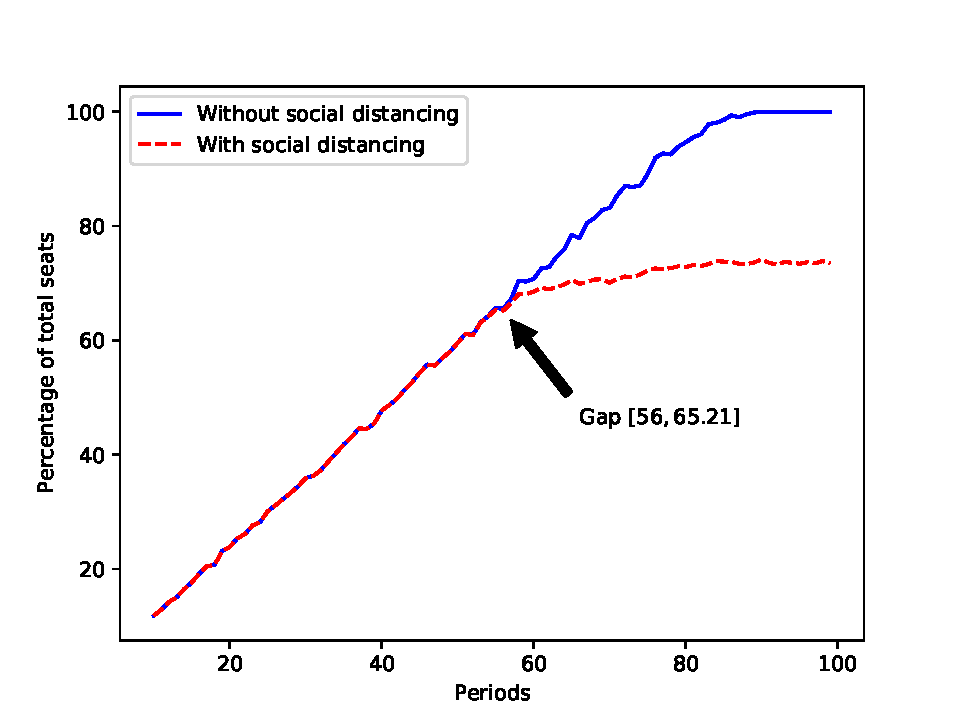
\includegraphics[width=0.48\textwidth]{./images/p1.pdf}}
            \subfigure[When $\gamma =1.9$]{
              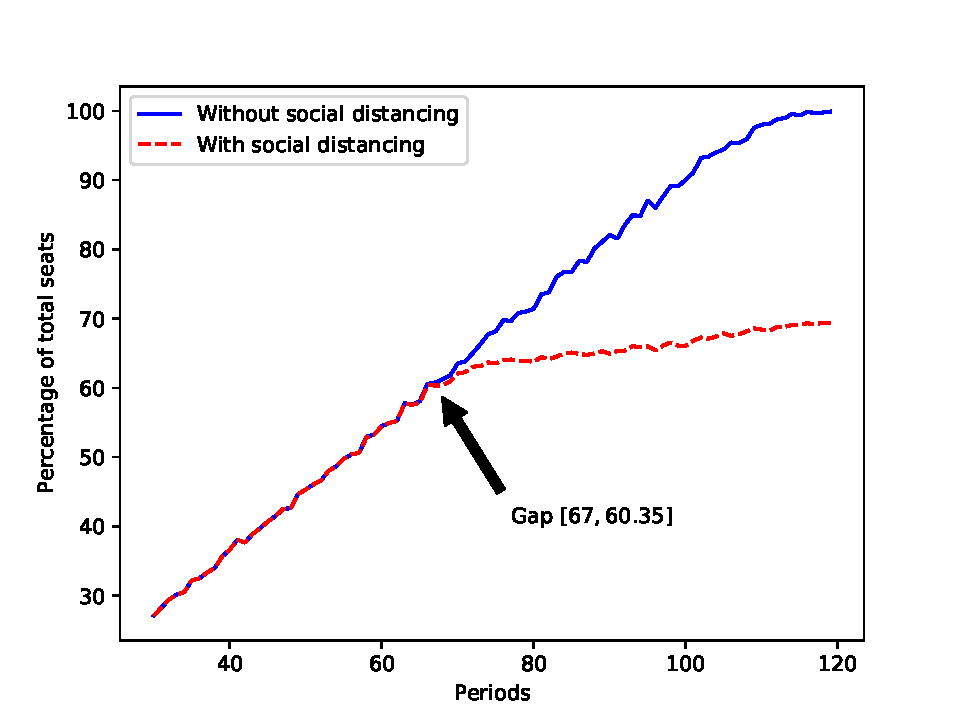
\includegraphics[width=0.48\textwidth]{./images/p2.pdf}}
          \end{figure}
        \scriptsize
        The gap point represents the first period where the number of people without social distancing is larger than that with social distancing and the gap percentage is the corresponding percentage of total seats.
    \end{frame}
      
    \begin{frame}{Estimation of Gap Point}
      \begin{figure}[ht]
        \centering
        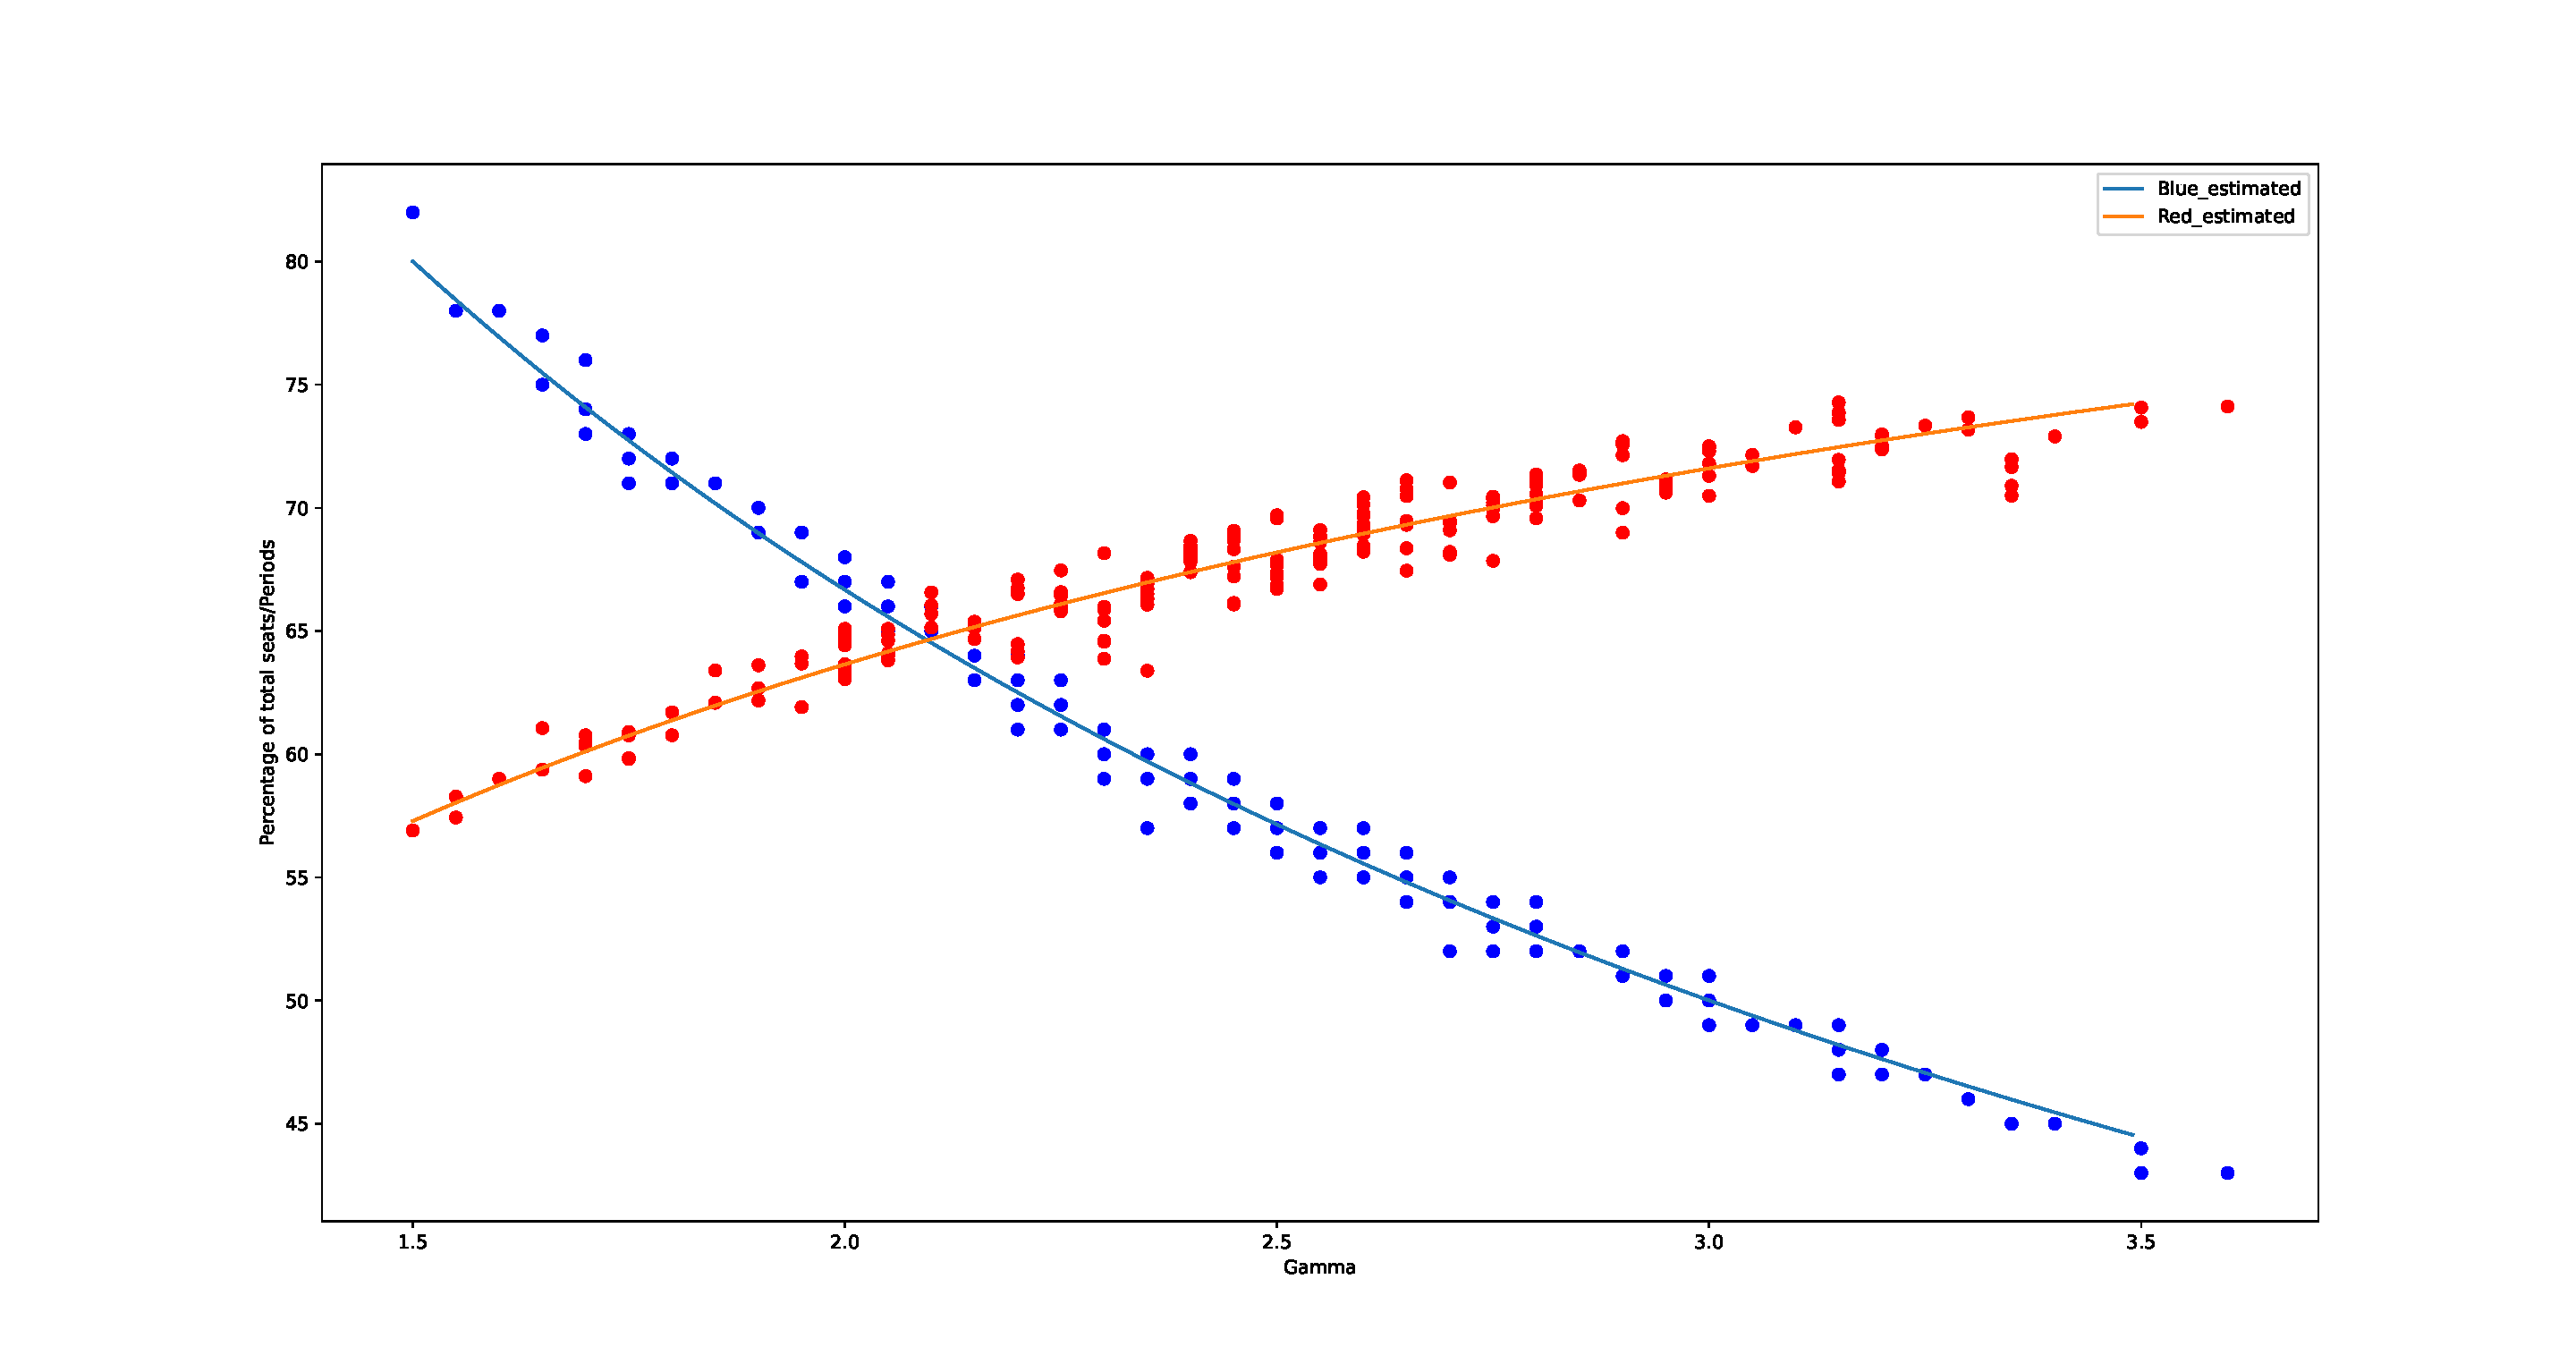
\includegraphics[width = 0.8\textwidth]{./images/gamma_estimation.pdf}
        \caption{Gap points under 200 probabilities}
    \end{figure}
    \scriptsize
    {\color{blue} Blue points}: period of the gap point.
    {\color{red} Red points}: occupancy rate of the gap point. 
    Gap points can be estimated.
    \end{frame}